% TeX root = ../main.tex

\chapter{Introduction to Modular Forms}

\vspace{-1em}
\begin{center}
\large\textbf{Abstract}
\end{center}

\noindent
This report studies the theory of modular forms and Jacobi forms, and their role in counting problems arising in the context of quantum black holes \cite{DMZ}. We begin with a brief review of Fourier series \cite{BrownNotes} and classical modular forms \cite{DiamondShurman}, before developing the theory of modular forms for congruence subgroups and Jacobi forms. We then discuss their applications to string theory, including a correspondence between type IIA string theory on $K3 \times T^2$ and the heterotic string on $T^4 \times T^2$ at the level of partition functions. We also give a physical interpretation of the Fourier coefficients of $1/\Delta$ (see Appendix~\ref{app:Asymptotics}).

\vspace{0.5em}
\noindent\rule{\textwidth}{0.4pt}


\section{Fourier Series}

Let $\mathcal{S}$ denote the space of complex-valued, $\mathbb{Z}$-periodic functions on $\mathbb{R}$. Let the inner product be the standard Hermitian inner product \cite[Section~1.2]{BrownNotes}. For $f \in \mathcal{S}$, define the Fourier coefficients
\[
c_n(f) := \int_0^1 f(x)e^{-2\pi i n x}\,dx, \quad n \in \mathbb{Z}.
\]
The Fourier series of $f$ is then
\[
f(x) \sim \sum_{n\in\mathbb{Z}} c_n(f)\,e^{2\pi i n x}.
\]

\section{Modular Forms}
\subsection{Basic Definitions and Results}

% \defn{Upper Half Plane $\bbH$}{$$\bbH:=\{z\in \bbC: im(z)>0\}$$}
% \defn{$SL(2,\bbR)$}{$$SL(2,\bbR):=\bigg\{M=\bigg{(}\begin{matrix}a & b \\ c &d \end{matrix}\bigg{)}: a,b,c,d \in \bbR \textbf{ and } ad-bc=1 \bigg\} $$}
% \defn{$GL(2,\bbR)$}{$$GL(2,\bbR):=\bigg\{M=\bigg{(}\begin{matrix}a & b \\ c &d \end{matrix}\bigg{)}: a,b,c,d \in \bbR \textbf{ and } ad-bc\neq 0 \bigg\} $$}
% \defn{$GL^+(2,\bbR)$}{$$GL^+(2,\bbR):=\bigg\{M=\bigg{(}\begin{matrix}a & b \\ c &d \end{matrix}\bigg{)}: a,b,c,d \in \bbR \textbf{ and } ad-bc>0\bigg\} $$}
\begin{definition}[Basic objects]
\[
\mathbb{H}=\{z\in\mathbb{C}:\operatorname{Im}(z)>0\}\] 
\[SL_2(\mathbb{R})=\{A\in M_2(\bbR):\det A=1\}\] 
\[GL_2(\mathbb{R})=\{A\in M_2(\bbR):\det A\neq0\}\]
\[GL_2^+(\mathbb{R})=\{A\in M_2(\bbR):\det A>0\}.\]
\end{definition}


% We have rather trivially the following inclusions
% $$SL(2,\bbR)\hookrightarrow GL^+(2,\bbR) \hookrightarrow GL(2,\bbR) $$

\begin{definition}[Modular form for $SL_2(\bbZ)$]
Let $k \in \bbZ$. A function $f:\bbH \to \bbC$ is a modular form of weight $k$ if:
\[
f\!\left(\frac{az+b}{cz+d}\right) = (cz+d)^k f(z)
\quad \forall 
\begin{pmatrix} a & b \\ c & d \end{pmatrix} \in SL_2(\bbZ),\ z \in \bbH,
\]
and $f$ is holomorphic on $\bbH$ and bounded as $\operatorname{Im}(z)\to\infty$.
\end{definition}

\corp{
For $f \in M_k(SL_2(\bbZ))$,
\[
f(z+1)=f(z),\quad f(-1/z)=z^k f(z),\quad f(z)=(-1)^k f(z).
\]
In particular, if $k$ is odd then $f\equiv 0$.
}{
Since $T, S, -I \in SL_2(\bbZ)$, the result follows.
}

\fact\label{fact of generation of SL}{$SL(2,\bbZ)$ is generated by $\bigg(\begin{matrix}1&1 \\0&1 \end{matrix}\bigg) $ and $ \bigg(\begin{matrix}0&-1 \\1&0 \end{matrix}\bigg) $. \cite[Theorem~3.3]{KonradNotes} }

% \begin{corollary}
%   Since $f$ is $\bbZ$ periodic, and holomorphic, we can fourier expand $f$, which gives $$f(x+iy)=\sum_{n \in \bbZ} a_n e^{2\pi i n (x+iy)}=\sum_{n\in \bbZ} a_n e^{2\pi i nx}e^{-2\pi n y} $$
%   If $a_n$ for negative $n$ were to be non zero, we would have that $f$ is unbounded as $y\to \infty$ (since $e^{2\pi n y}$ would go unbounded). Therefore, $\forall n<0, a_n=0$. $a_0$ can be $0$, in which case $\lim_{y\to \infty} f(x+iy)=a_0=0$. If $a_0=0$, then the modular form is called a \textbf{Cusp Form}.\label{cusp form} 
% \end{corollary}
\begin{definition}[Weakly holomorphic modular forms]
A function $f:\bbH \to \bbC$ is a weakly holomorphic modular form of weight $k$ if
\[
f\!\left(\frac{a\tau+b}{c\tau+d}\right) = (c\tau+d)^k f(\tau)
\]
for all $\begin{pmatrix}a & b \\ c & d\end{pmatrix} \in SL_2(\bbZ)$, and $f$ is holomorphic on $\bbH$ with a Fourier expansion
\[
f(\tau) = \sum_{n\ge -N} a_n q^n, \quad q = e^{2\pi i \tau},
\]
for some $N \ge 0$.
\end{definition}

\begin{definition}
Let $M_k$, $S_k$, and $M_k^!$ denote respectively the spaces of modular forms, cusp forms, and weakly holomorphic modular forms of weight $k$ (all over $\bbC$). Thus,
\[
S_k \subset M_k \subset M_k^!.
\]
\end{definition}

\begin{remark}
When necessary, we specify the group, e.g. $M_k(SL_2(\bbZ))$ or $S_k(SL_2(\bbZ))$.
\end{remark}

\subsubsection{Growth of Fourier coefficients ($SL_2(\bbZ)$)}

For $f(\tau)=\sum a_n q^n$, we have:
\[
\begin{aligned}
f \in S_k &\implies a_n = O(n^{k/2}),\\
f \in M_k &\implies a_n = O(n^{k-1}),\\
f \in M_k^! &\implies a_n = O(e^{C\sqrt{n}})
\end{aligned}\]
\cite{DMZ} \cite[Section~5]{KonradNotes}.


\defn{Eisenstein Series $E_k$}{$$E_k(z):=\sum_{(m,n)\in \bbZ^2, (m,n)\neq 0}\frac{1}{(mz+n)^k}$$}
\begin{remark}
  $E_k(z)$ is a modular form of weight $k$ (for $SL_2(\bbZ)$) for all $k\geq 4$. They are very important examples of modular forms for they, in some sense, form the "building blocks" to construct other modular forms.

\end{remark}
\defn{Discriminant function $\Delta$}{ $$\Delta(z):= q \Pi_1^{\infty} (1-q^n)^{24} $$ (Where $q=e^{2\pi i z}$). This function is a \emph{cusp form} of weight 12.}
\defn{Dedekind Eta Function $\eta$}{ $$\eta(z):= q^{1/24} \Pi_1^{\infty} (1-q^n) $$ (Where $q=e^{2\pi i z}$). This function is a \emph{weakly holomorphic form} of weight $1/2$. For more discussion, see \cite[Section~3.9]{HokerKaidi}.}

\subsection{Structure of $M_k(SL_2(\bbZ))$ and $S_k(SL_2(\bbZ))$}

{We present, without proof, one of the cornerstone theorems in Modular Forms theory:}

\thmp{Structure Theorem}{\label{mk vs mk-12} \begin{enumerate}
  \item $M_k(SL_2(\bbZ))$ is generated by the monomials $E_4^{\alpha}E_6^{\beta}$ such that $4\alpha+6\beta=k$. In other words, as a vector space we see that $$M_k(SL_2(\bbZ))=\langle\{E_4^{\alpha}E_6^{\beta}:4\alpha+6\beta=k \ (\text{ in integers}) \} \rangle$$ A trivial corollary of this is that, $M_k(SL_2(\bbZ))$ is a finite dimensioned vector space.
  \item $$M_*(SL_2(\bbZ))=\oplus_k M_k(SL_2(\bbZ))$$ forms a \emph{Graded Algebra-} A direct sum of submodules that forms an algebra. Moreover, $$M_*(SL_2(\bbZ))=\bbC[E_4,E_6]$$ This says that, in principle, the space of all modular forms for $SL_2(\bbZ)$ acts as the set of all 2 variable polynomials over $\bbC$ ($E_4$ and $E_6$ are algebraically independent). 
  \item \label{mk vs ek and sk} $$M_k(SL_2(\bbZ))=\bbC \cdot E_k+S_k$$ This result says that every modular form is some scalar times the Eisenstein, with the "error term" being a cusp form (or the other way around, where every modular form is a cusp form, with the error term being a factor of the Eisenstein)
  \item \label{sk vs mk-12}$$S_k=\Delta \cdot M_{k-12}$$
\end{enumerate}}{\cite[Section~5]{KonradNotes}, and \cite[Theorem~3.9]{BrownNotes}(The Riemann-Roch Theorem) discuss this in greater detail.}


\begin{remark}
  With the results \ref{mk vs ek and sk} and \ref{sk vs mk-12} of \ref{mk vs mk-12}, we see that $M_k=\bbC E_k+\Delta M_{k-12}=\bbC E_k+\Delta (\bbC E_{k-12}+\Delta M_{k-24})=\bbC E_k+\Delta (\bbC E_{k-12} + \Delta(\bbC E_{k-24}+\Delta M_{k-36}))=\cdots $ from which we get that any modular form $f$ of weight $k$ can be written as $$ f=\sum_{n=0}^{[k/12]}\alpha_n E_{k-12n} \Delta^n$$
\end{remark}
\subsection{Fundamental Domain and the action of $SL_2(\bbZ)$ on $\bbH $}
The defining action of a $\gamma=\begin{bmatrix}
  a \ b \\ c \ d  
\end{bmatrix} \in SL_2(Z)$ on a vector $z \in \bbH $ is given by: $$ z \mapsto \gamma z=\frac{az+b}{cz+d}$$
% Note the following fact: $$\operatorname{im}(\frac{az+b}{cz+d})=\frac{(ad-bc) \operatorname{im}(z)}{|cz+d|^2} $$  

% In order to stay in $\bbH$, we are forced to use $GL_2^+(\bbR)$. The need for $SL_2(\bbZ)$ comes from analysing Lattices of the form $\omega_1 \bbZ \oplus \omega_2 \bbZ$ (for $\omega_1,\omega_2 \in \bbR^2$). A change of basis of the lattice corresponds to a $SL_2(\bbZ)$ multiplication.
% \newline Since $\begin{bmatrix}
%   1 \ 1 \\ 0 \ 1  
% \end{bmatrix} \text{ and }\begin{bmatrix}
%   0 \ -1 \\ 1 \ 0  
% \end{bmatrix}  \in SL_2(\bbZ)$, the respective actions are $z \mapsto z+1$ (translations) and $z \mapsto -1/z$ (inversions). 

\begin{definition}[Fundamental domain for $\Gamma \le SL_2(\bbZ)$]
A subset $\mathcal{F}\subset\bbH$ is a fundamental domain for $\Gamma$ \cite{PrasadNotes} if $\bbH=\bigcup_{\gamma\in\Gamma}\gamma\mathcal{F}$, $(\gamma_1\mathcal{F})^\circ\cap(\gamma_2\mathcal{F})^\circ=\varnothing$ for $\gamma_1\neq\gamma_2$, and $\mathcal{F}=\overline{\mathcal{F}^\circ}$.
\end{definition}

\begin{example}
  A fundamental Domain for $SL_2(\bbZ)$ is $$\mathcal F_{SL_2(\bbZ)}:=\{x \in \bbH: |\operatorname{Re}(x)|\leq \frac{1}{2} \text{ and }|x|>1 \} $$
\end{example}

% TIKZ PICTURE %

\begin{center}
\begin{tikzpicture}[scale=1.5]\label{fundamental_domain}

% Axes
\draw[->] (-1.5,0) -- (1.5,0) node[right] {$\Re(\tau)$};
\draw[->] (0,-0.1) -- (0,2.0) node[above] {$\Im(\tau)$};

% Shaded fundamental domain
\fill[red!30, opacity=0.6]
  (-0.5, 1.8)
  -- (-0.5, 0.866)
  arc[start angle=120, end angle=60, radius=1]
  -- (0.5, 1.8)
  -- cycle;

% Boundary lines Re(tau) = ±1/2, drawn only from arc upward
\draw[thick] (-0.5, 0.866) -- (-0.5, 1.8);
\draw[thick] ( 0.5, 0.866) -- ( 0.5, 1.8);

% Unit circle arc from 120° to 60°
\draw[thick] (-0.5, 0.866) arc[start angle=120, end angle=60, radius=1];

% Dashed extensions below the domain (for context)
\draw[dashed, gray] (-0.5, 0) -- (-0.5, 0.866);
\draw[dashed, gray] ( 0.5, 0) -- ( 0.5, 0.866);
\draw[dashed, gray] (-0.5, 0.866) arc[start angle=120, end angle=180, radius=1];
\draw[dashed, gray] ( 0.5, 0.866) arc[start angle=60,  end angle=0,   radius=1];

% Tick marks and labels on x-axis
\draw (-0.5, 0.03) -- (-0.5,-0.03) node[below] {$-\tfrac{1}{2}$};
\draw ( 0.5, 0.03) -- ( 0.5,-0.03) node[below] {$\tfrac{1}{2}$};
\draw ( 1.0, 0.03) -- ( 1.0,-0.03) node[below] {$1$};
\draw (-1.0, 0.03) -- (-1.0,-0.03) node[below] {$-1$};

% Special points
\fill (0, 1) circle (1pt) node[right] {$i$};
\fill ({cos(60)}, {sin(60)}) circle (1pt) node[above right] {$e^{i\pi/3}$};
\fill ({cos(120)}, {sin(120)}) circle (1pt) node[above left] {$e^{2i\pi/3}$};

% Label
\node at (0, 1.35) {$\mathcal{F}$};

\end{tikzpicture}
\end{center}

%TIKZ PICTURE ENDS
\subsection{Shimura slash operator}

For $\gamma=\begin{pmatrix}a&b\\c&d\end{pmatrix}\in GL_2^+(\bbQ)$,
\[
(f|_k\gamma)(z)=(\det\gamma)^{k/2}(cz+d)^{-k}f\!\left(\frac{az+b}{cz+d}\right),
\]
with $(f|_k\gamma_1)|_k\gamma_2=f|_k(\gamma_1\gamma_2)$ \cite[p.~9]{PrasadNotes}.
\begin{comment}
\subsubsection{What are Cusps?}
We first look at the map $(x,y)=z\mapsto e^{2\pi i z}=e^{2\pi i x}e^{-2\pi y}$. This maps the upper half plane to the punctured open unit disc ($y\to 0$ maps to the $|x|=1$ boundary, and $i\infty$ (which is $\infty $, specifically reached through, $\lim(y)\to \infty$)) maps to 0. $q=e^{2\pi i z}=0$ corresponds to $z=i \infty$ (the specific $\infty$ reached through $\lim y \to \infty$). Note that, the points on the boundary of the unit disc corresponds to $y \to 0$, which don't belong to the upper half plane. Hence, the image of $\bbH$ under $e^{2\pi i z}$ is not compact.

The problem is that, the upper half plane $\bbH$ is itself not compact. This can be made compact by adding a point $\infty$ and $\bbR$ and defining topologies as usual. This makes a compact Riemann Surface, but it is not the most viable choice for our goals with modular forms. 
This is where the topology $\Gamma/ \bbH$ comes into picture. Note that, 
$${SL_2(\bbZ)} / {\bbH}=\mathcal F=\{x \in \bbH: |\operatorname{Re}(x)|\leq 1/2 \text{ and }|x|>1\}$$

\subsubsection{What are Cusps?}

We begin by considering the map
\[
z = x + iy \mapsto q = e^{2\pi i z} = e^{2\pi i x} e^{-2\pi y}.
\]
Since $y > 0$, we have $0 < |q| < 1$, so this map sends the upper half-plane $\bbH$ to the punctured unit disk.

As $y \to \infty$, we see that $|q| = e^{-2\pi y} \to 0$. Thus the point $z = i\infty$ corresponds to $q = 0$. On the other hand, as $y \to 0^+$, we have $|q| \to 1$, so points approach the boundary of the unit disk.

This shows that the upper half-plane $\bbH$ corresponds to a punctured disk, with the missing point $q=0$ corresponding to $z = i\infty$.

Now consider first the action of $SL_2(\bbZ)$ on $\bbH$. The quotient space $SL_2(\bbZ)\backslash \bbH$ can be visualized using a fundamental domain $\mathcal{F} \subset \bbH$, for example:
\[
\mathcal{F} = \left\{ z \in \bbH : |\operatorname{Re}(z)| \le \tfrac{1}{2}, \ |z| \ge 1 \right\}.
\]
This space, however, is non compact. In order to compactify this space, (and viably include the relevant points, i.e. those that correspond to $q=0$ and $|q|=1$)
\end{comment}
\subsection{Congruence Subgroups of $SL_2(\bbZ)$ and Modular Forms for Congruence Subgroups}
\defn{$\Gamma(N)$}{For $N\in \bbN$, we define the principal congruence subgroup of level $N$ as $$\Gamma(N):=\bigg\{\bigg(\begin{matrix}a&b \\c&d \end{matrix}\bigg)\in SL_2(\bbZ): \bigg(\begin{matrix}a&b \\c&d \end{matrix}\bigg)\equiv \bigg(\begin{matrix}1&0 \\0&1 \end{matrix}\bigg) \textbf{ mod } N \bigg\} $$}
It is not difficult to show that $\Gamma(N)$ is a normal subgroup of $SL_2(\bbZ)$, and that the quotient group $SL_2(\bbZ)/\Gamma(N)$ is isomorphic to $SL_2(\bbZ/N\bbZ)$ (Hence, $\Gamma(N)$ is a finite index subgroup of $SL_2(\bbZ)$).
\defn{$\Gamma_0(N)$}{For $N\in \bbN$, we define the congruence subgroup of level $N$ as $$\Gamma_0(N):=\bigg\{\bigg(\begin{matrix}a&b \\c&d \end{matrix}\bigg)\in SL_2(\bbZ): c\equiv 0 \textbf{ mod } N \bigg\} $$}
\defn{$\Gamma_1(N)$}{For $N\in \bbN$, we define the congruence subgroup of level $N$ as $$\Gamma_1(N):=\bigg\{\bigg(\begin{matrix}a&b \\c&d \end{matrix}\bigg)\in SL_2(\bbZ): a\equiv d \equiv 1 \textbf{ mod } N \textbf{ and } c\equiv 0 \textbf{ mod } N \bigg\} $$}
\begin{remark}
  $\Gamma(N)\subset \Gamma_1(N) \subset \Gamma_0(N) \subset SL_2(\bbZ)$
\end{remark}
\defn{Modular Forms for $\Gamma$ (where $\Gamma$ is a congruence subgroup of $SL_2(\bbZ)$)}{Let $\Gamma$ be a congruence subgroup of $SL_2(\bbZ)$ and $k\in \bbZ$. A function $f:\bbH \to \bbC$ is a modular form of weight $k$ for $\Gamma$ if:
\begin{enumerate}
\item $f(z)|_k[\gamma]=f(z)$ for all $\gamma \in \Gamma$
\item $\forall \gamma \in SL_2(\bbZ)$, $f(z)|_k[\gamma]=\sum_{n\geq 0}a_n q^{n/N}$
\end{enumerate}
}
\begin{remark}
  The reason why we need the full $SL_2(\bbZ)$ in the second condition is that, we need to ensure that $f$ is holomorphic at all the cusps of $\Gamma$. For more on this, refer to Appendix~\ref{app:cusps} and \cite[Section~2.2]{MasdeuNotes}.
\end{remark}
We now briefly introduce Jacobi Forms:
\defn{Jacobi Forms}{Let $k,m \in \bbZ$. A holomorphic function $\phi: \bbH \times \bbC \to \bbC$ is a Jacobi form of weight $k$ and index $m$ if:
\begin{itemize}
\item $\phi(\frac{a\tau+b}{c\tau+d}, \frac{z}{c\tau+d})=(c\tau+d)^k e^{2\pi i m \frac{cz^2}{c\tau+d}} \phi(\tau,z)$ for all $\bigg(\begin{matrix}a&b \\c&d \end{matrix}\bigg) \in SL_2(\bbZ)$
\item $\phi(\tau, z+\lambda \tau + \mu)=e^{-2\pi i m (\lambda^2 \tau + 2\lambda z)} \phi(\tau,z)$ for all $\lambda, \mu \in \bbZ$
\item $\phi(\tau,z)=\sum_{n,r} c(n,r) q^n \zeta^r$ where $q=e^{2\pi i \tau}$ and $\zeta=e^{2\pi i z}$, and $c(n,r)=0$ unless $4nm \geq r^2$ (This condition is called the "holomorphicity condition" and ensures that $\phi$ is holomorphic at all the cusps of the Jacobi group).
\end{itemize}}
